\newpage
%%%%%Caso de Uso
		\hypertarget{Gestion de Categorias}{}
		\section{\textbf{Caso de uso CU01 - Gesti\'on de Categorias}}

			\subsection{Descripci\'on}
				\textsl{Caso de uso que describe la gesti\'on de la una \hyperlink{Categoria}{categor\'ia} incluye a los casos de uso, ver categor\'ia, registrar categor\'ia, modificar categor\'ia, eliminar categor\'ia y buscar categor\'ia. \\ \\}
			\subsection{Diagrama}
				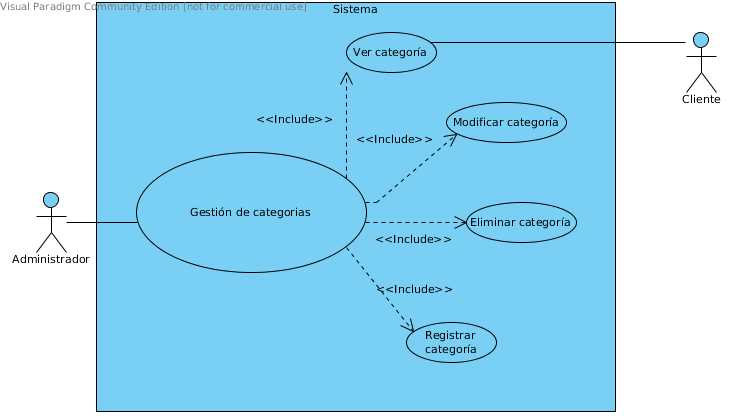
\includegraphics[scale=0.9]{images/casos/gestionCategoria.png}
				
			\subsubsection{ \textbf{Atributos relevantes} }

				\begin{longtable}{p{4cm}|p{11cm}}
				\hline
					{Caso de Uso}&{Gesti\'on de categor\'ias}\\
				\hline
					{\hyperlink {Autor}{Actor}}&{Gerar Haran Rodr\'iguez Molina}\\
				\hline
					{\hyperlink {Reviso}{Revis\'o}}&{Marco Polo Navarrete \'Alvarez}\\
				\hline
					{\hyperlink {Prioridad}{Prioridad}}&{Alta}\\
				\hline
					{\hyperlink {Madurez}{Madurez}}&{Alta}\\
				\hline
					{\hyperlink {Estatus}{Estatus}}&{Aprobado}\\
				\hline
					{\hyperlink {Proposito}{Prop\'osito}}&{Gestionar las categor\'ias que puedan formar parte de SpaceShop.}\\
				\hline
					{\hyperlink {Actor}{Actor}}&{\hyperlink{Cliente}{Cliente} }\\
				\hline
					{\hyperlink {Entradas}{Entradas}}&{ 
					\begin{itemize}
						\item[?] Solicitud de registrar categori\'ia.
						\item[?] Solicitud de eliminar categori\'ia.
						\item[?] Solicitud de modificar categori\'ia.
						\item[?] Solicitud de ver categori\'ia.
					\end{itemize}	 
					}\\
				\hline
					{\hyperlink {Salidas}{Salidas}}&{
					\begin{itemize}
						\item[?] Una nueva categor\'ia registrada en el sistema.
						\item[?] Modificaci\'on de una categor\'ia registrada en el sistema.
						\item[?] Eliminaci\'on de una categor\'ia registrada en el sistema.
						\item[?] Mensaje de Confirmaci\'on.
						\item[?] Mensaje de Error.
					\end{itemize}		
					}\\

				\hline
					{\hyperlink {Precondiciones}{Precondiciones}}&{
					\begin{itemize}
						\item[?] Cargar lo cat\'alogo de CATEGORIAS.
						\item[?] Cargar lo cat\'alogo de USUARIO.
						\item[?] Que la categor\'ia a registrar a\'un no est\'e registrada en el sistema.
						\end{itemize}	
					}\\

				\hline
					{\hyperlink {Postcondiciones}{Postcondiciones}}&{
					\begin{itemize}
						\item[?] Que la categor\'ia registrada pueda visualizarse en el sistema.
						\item[?] Que la categor\'ia modificada pueda visualizarse en el sistema.
						\item[?] Que la categor\'ia eliminada ya no pueda visualizarse en el sistema por parte del \hyperlink{Cliente}{Cliente}.
						\end{itemize}
						}\\
				\hline
					{\hyperlink {Errores}{Errores}}&{
					\begin{itemize}
						\item[?] La categor\'ia a registrar ya existe.
						\item[?] La categor\'ia a eliminar no se permite gracias a la \hyperlink{RN002}{RN002}.
					\end{itemize}		
					}\\
				\hline
					{\hyperlink {Observaciones}{Observaciones}}&{La gesti\'on de categor\'ias solo la podr\'a realizar el \hyperlink{Administrador}{Administrador}, el usuario solo podr\'a visualizar las categor\'ias que se encuentran registradas en el sistema\\}
				\end{longtable}

%%%%%%%Trayectorias
\newpage
	\subsection {Trayectoria Principal}
		\begin{enumerate}
			\item \UCactor selecciona el men\'u "Dar de alta usuario".
			\item \UCsist despliega pantalla \hyperlink{AU-I1}{AU-I1}, que contiene los campos requeridos para el registro.
			\item \UCactor Llena los campos de acuerdo al \hyperlink{MC}{modelo conceptual} 
			\item \UCactor Env\'ia los datos presionando el bot\'on   Enviar.
			\item \UCsist El sistema los valida de acuerdo a la regla del negocio \hyperlink {AU-RN1} {AU-RN1}
			\item \UCsist Muestra en pantalla los datos del nuevo registro creado.
			\item \UCactor Presiona el bot\'on "Aceptar".
			\item \UCsist Regresa a la pantalla de inicio.
			\\
			\\
			----Fin del Caso de Uso
		\end{enumerate}

	%%%%%%%%%%%Trayectorias Aternativas
	\subsection {Trayectoria Alternativa A}
		Condici\'on: Presiona el bot\'on cancelar en la interfaz Dar alta usuario.
			\\
		\begin{enumerate}
			\item Presiona el bot\'on Cancelar.
			\item Regresa al paso 3 de la trayectoria principal.
			\\
			Fin de la trayectoria.
			\\
		\end{enumerate}